\documentclass[svgnames]{beamer}
%\usepackage[usenames,dvipsnames,svgnames,table]{xcolor}
% \mode<presentation>{\usetheme{Ilmenau}} % Ilmenau
% \mode<presentation>{\usetheme{Warsaw}} % Warsaw
\mode<presentation>{\usetheme{Darmstadt}} % Darmstadt
% behaviors

% toc before each section
% \AtBeginSection[]
% {
% \begin{frame}{Table of Contents}
% \tableofcontents[currentsection]
% \end{frame}
% }

% \AtBeginSection{\frame{\sectionpage}}
% \AtBeginSubsection{\frame{\subsectionpage}}
% \AtBeginSubsubsection{\frame{\subsubsectionpage}}

% add number of page
\beamertemplatenavigationsymbolsempty
\setbeamerfont{page number in head/foot}{}
\setbeamertemplate{footline}[frame number]

% add number of page
% \addtobeamertemplate{navigation symbols}{}{%
%     \usebeamerfont{footline}%
%     \usebeamercolor[fg]{footline}%
%     \hspace{1em}%
%     \insertframenumber/\inserttotalframenumber
% }

% remove symbols
\setbeamertemplate{navigation symbols}{}

% headers
\title{CSRF attack: even Google was vulnerable.}
\author{Quentin Lemaire \& David Kufa}
\date{\today}

% content
\begin{document}
  
\maketitle % build title

% Hello,
% This presentation will be about:
% ...

% introduction
\section*{Introduction}
\begin{frame}
\frametitle{Introduction}
\begin{itemize}
  \item \textit{Cross-Site Request Forgery} (CSRF) also known as ``sea surf''
  \item Mix of theoretical \& practical explanations about CSRF.
  \item Presentation of 2 Google stories related to CSRF
\end{itemize}

\end{frame}

% toc => be really short (maybe don't speak about toc since it's
% explained in introduction

% CSRF:
% - What is it ? How it works ? How to identify it ?
% - How to exploit it ? How to prevent it ?
% Google stories:
% - Description
% (- Exploitation) really fast
% - Impact (different !)
\begin{frame}
  \frametitle{Summary}
  \tableofcontents
\end{frame}

%% ------- %%

\section{CSRF}
% \begin{frame}
%   \frametitle{CSRF}
%   \tableofcontents[currentsection]
% \end{frame}

% description
\subsection{What is it ?}
\begin{frame}
  \frametitle{What is CSRF ?}
  
  \begin{itemize}
   \item Web vulnerability discovered in 2001
   \item Top 8 from OWASP\footnote{\textit{Open Web Application 
       Security Project}: \url{https://www.owasp.org/}} most critical 
   web application security risks in 2013
   \item Uses victims' lack of knowledge \& websites vulnerability
  \end{itemize}
  
  \pause
  
  \begin{block}{Idea of the attack}
    Forging fake HTTP(S) requests in order to execute legitimate actions on the 
    authenticated victim's behalf.
  \end{block}

% C. Shiflett said (compared to XSS) : "Cross-Site Request Forgeries are an almost 
% opposite style of attack. Rather than exploiting the trust that a user has for a 
% website, they (CSRF attacks) exploit the trust that a website has for a user"


% alertblock
% exampleblock
%   \begin{block}{CSRF}
%     Sea surf uiuiui
%   \end{block}
\end{frame}

% Scheme:
% 1- Real authentication from the client to the vulnerable web server
% 2- Server authenticates the user and sets up cookie
% 3- Victim surfs on the internet & visits the attacker website (via 
% social engineering, Cross-Site Scripting (XSS) web vulnerability, ...)
% 4- Attacker webserver answers with malicious page embeding malicious 
% code (HTML, JavaScript, etc.)
% 5- Code is executed (interpreted) by the browser's victim and a request 
% can be sent on the user's behalf (with his or her credentials)

\subsection{How it works ?}
\begin{frame}
  \frametitle{Concrete scenario}
  \begin{figure}[h!t]
  \begin{center}
    \only<1>{\fbox{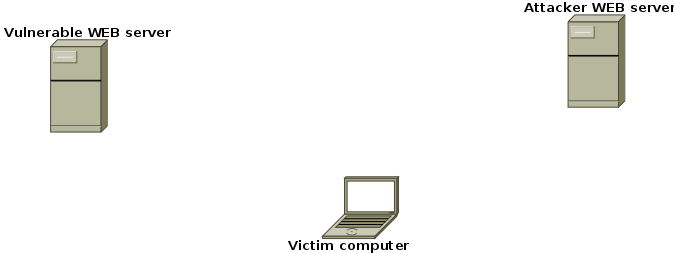
\includegraphics[width=\textwidth]{media/CSRF_attack_0.png}}} % actors
    \only<2>{\fbox{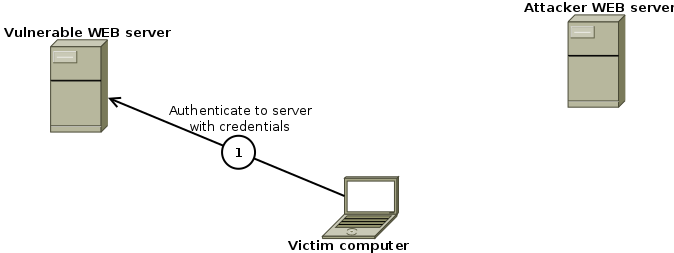
\includegraphics[width=\textwidth]{media/CSRF_attack_1.png}}} % 1
    \only<3>{\fbox{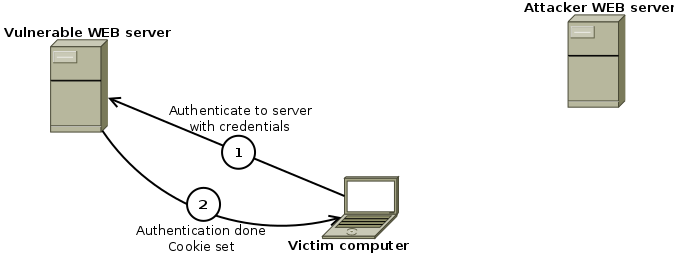
\includegraphics[width=\textwidth]{media/CSRF_attack_2.png}}} % 2
    \only<4>{\fbox{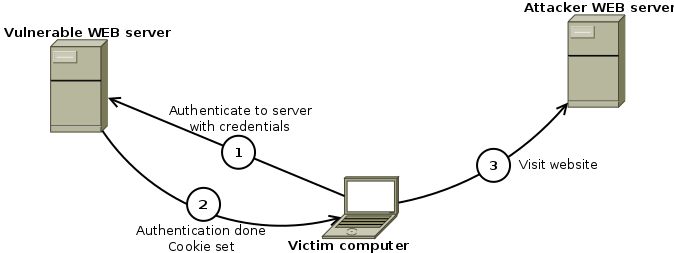
\includegraphics[width=\textwidth]{media/CSRF_attack_3.png}}} % 3
    \only<5>{\fbox{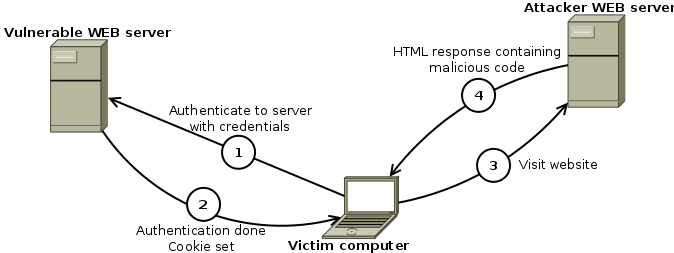
\includegraphics[width=\textwidth]{media/CSRF_attack_4.png}}} % 4
    \only<6>{\fbox{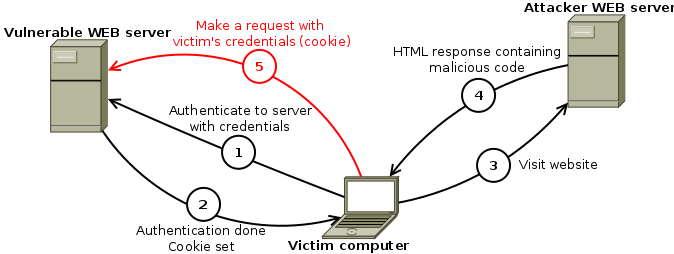
\includegraphics[width=\textwidth]{media/CSRF_attack_5.png}}} % 5
    \only<7>{\fbox{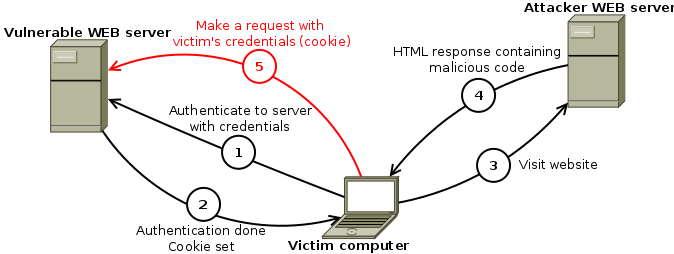
\includegraphics[width=0.9\textwidth]{media/CSRF_attack_5.png}}} % 5 small
       
    \caption{
      CSRF attack scenario.
      \tiny{\textit{Realized with Dia: \url{https://wiki.gnome.org/Apps/Dia/}.}}
    }
  \end{center}
  \end{figure}
  
  \only<7>{
   Example of malicious code:
  \texttt{<img src="http://vulnerable-website.com/?\textcolor{red}{action=deleteAccount}" width=0 height=0 />}
  }
\end{frame}

\begin{frame}
 \frametitle{Practical example}
 
 % We're gonna show you samples of vulnerable services in the webapp we developped
 
 \begin{center}
    % TODO insert video vulnerable
    \tiny{\textit{This web application has been developed by Quentin Lemaire \& David Kufa. Source is accessible on Github: \url{https://github.com/Groscheri/csrf-seminar/tree/master/webapp}}}
 \end{center}
\end{frame}


\subsection{How to prevent it ?}
% exploitation & prevention
\begin{frame}
  \frametitle{Prevention} % webapp built from scratch
  % TODO text instead of video
  \begin{itemize}
   \item One-time tokens generated by the server
   \begin{itemize}
    \item Stored  % in session
    \item Signed  % with Hash Message Authentication Code (HMAC)
   \end{itemize}
   \item Double authentication % retype password for critical services or CAPTCHA
   \item Check HTTP-REFERER % where the request comes from

  \end{itemize}

  % TODO insert video none vulnerable ==> maybe not necessary since we don't have too much time
  % TODO if video => \tiny{\textit{This web application has been developed by Quentin Lemaire \& David Kufa. Source is accessible on Github: \url{https://github.com/Groscheri/csrf-seminar/tree/master/webapp}}}
\end{frame}


%% ------- %%


\section{Google was vulnerable}
\begin{frame}
  \frametitle{Google was vulnerable}
  \tableofcontents[currentsection]
\end{frame}
	
\begin{frame}
  \frametitle{Description}
  
  \begin{figure}
    
\includegraphics[width=.6\textwidth]{media/gmail_logo.png}
  \end{figure}	  
  
  \begin{itemize}
    \item Google's email service Gmail launched in 2007
    \pause
    \item First CSRF attack commenced on Gmail (January 2007)
    \pause
    \item \textbf{All your contacts are belong to us!}
    \item Contact list spoofing
    \begin{itemize}
      \item Phishing attempts and spam
    \end{itemize}
  \end{itemize}
\end{frame}

\begin{frame}
  \frametitle{Exploitation}
  \begin{itemize}
    \item JavaScript callback function returned all contacts
    \item Triggered when showing all available Gmail contacts
    \pause
    \item "Keep me logged in" - Cookie duration set to infinite
    \pause
    \item Even simple popups could be dangerous!
  \end{itemize}
\end{frame}

\subsection{Story 2}

\begin{frame}
  \frametitle{Description}
  
  \begin{figure}
    
\includegraphics[width=.6\textwidth]{media/gmail_logo_0.jpg}
  \end{figure}	  
  
  \begin{itemize}
    \item Back to the future - second CSRF attack (August 2007)
    \pause
    \item \textbf{All your accounts are belong to us!}
    \item Email filter hijacking
    \begin{itemize}
      \item Reading all emails and taking over accounts
    \end{itemize}
  \end{itemize}
\end{frame}

\begin{frame}
  \frametitle{Exploitation}
  \begin{itemize}
    \item Special form (multipart/form-data POST) used
    \item Injected with JavaScript by sending in the form
    \pause
    \item Setting new filter which redirects emails to new address
    \item Filter redirected both old and new emails to attacker
    \pause
    \item \textbf{Worked on almost every Gmail interface - harder for end-users to protect themselves}
  \end{itemize}
\end{frame}

\subsection{Conclusion of stories}

\begin{frame}
  \frametitle{Impact}
  \begin{itemize}
    \item Two serious security breaches
    \item Gmail newly released with 80.000 users
    \pause
    \item Result:
    \begin{itemize}
      \item neglectable impact
    \end{itemize}
    \pause
    \item Thought:
    \begin{itemize}
      \item How would it have turned out today with 900 million users?
    \end{itemize}
  \end{itemize}
\end{frame}

\section*{Conclusion}
\begin{frame}
  \frametitle{Our recommendations}
  \begin{itemize}
   \item Users
   \pause
   \begin{itemize}
    \item Disconnect from websites
    \item Be careful when you click on URL % received by email most of the time
    \item Use several browsers (or extension to disable JavaScript\footnote{NoScript for instance: \url{https://noscript.net/}})
   \end{itemize}
   \pause
   \item Developers
   \begin{itemize}
    \item Methods presented previously: tokens, referer, CAPTCHA, etc.
    \pause
    \item \textcolor{ForestGreen}{Use robust \textbf{frameworks}!} % well-known & tested (often developed by companies or open-source community)
   \end{itemize}

  \end{itemize}
\end{frame}


\begin{frame}
  \frametitle{Thanks}
  \begin{center}
    Thank you very much for your attention!
  \end{center}
\end{frame}


\end{document}